\documentclass[11pt,a4paper,twoside]{tesis}
% SI NO PENSAS IMPRIMIRLO EN FORMATO LIBRO PODES USAR
%\documentclass[11pt,a4paper]{tesis}

\usepackage{graphicx}
\usepackage{float}
\usepackage{titlesec}
\usepackage{hyperref}

\usepackage[dvipsnames]{xcolor}
\usepackage{listings}
\lstloadlanguages{Ruby}
\lstset{%
basicstyle=\ttfamily\color{black},
commentstyle = \ttfamily\color{red},
keywordstyle=\ttfamily\color{blue},
stringstyle=\color{orange}}

\definecolor{light-gray}{gray}{0.95}
\lstset{columns=fullflexible, showspaces=false, basicstyle=\ttfamily,
    backgroundcolor=\color{light-gray},xleftmargin=1cm,frame=lr,framesep=8pt,framerule=0pt}


\usepackage[utf8]{inputenc}
\usepackage[spanish]{babel}
\usepackage[left=3cm,right=3cm,bottom=2cm,top=2cm]{geometry}
\setcounter{tocdepth}{5}
\setcounter{secnumdepth}{5}%Should do the work for the subsubsection, but it doesn't

\begin{document}

%%%% CARATULA
\def\titulo{Licenciado }

\def\autor{Andrés Laurito}
\def\tituloTesis{Haikunet: \mbox{SDN programming language}}
\def\runtitulo{Haikunet: a SDN programming language for debugging the network}
\def\runtitle{Haikunet: SDN programming language}
\def\director{Hernán Melgratti}
\def\codirector{Rodrigo Castro}
\def\lugar{Buenos Aires, 2017}
\newcommand{\HRule}{\rule{\linewidth}{0.2mm}}
%
\thispagestyle{empty}

\begin{center}\leavevmode

\vspace{-2cm}

\begin{tabular}{l}

\includegraphics[width=2.6cm]{logofcen.pdf}
\end{tabular}


{\large \sc Universidad de Buenos Aires

Facultad de Ciencias Exactas y Naturales

Departamento de Computaci\'on}

\vspace{6.0cm}

%\vspace{3.0cm}
%{
%\Large \color{red}
%\begin{tabular}{|p{2cm}cp{2cm}|}
%\hline
%& Pre-Final Version: \today &\\
%\hline
%\end{tabular}
%}
%\vspace{2.5cm}

{\huge\bf \tituloTesis}

\vspace{2cm}

{\large Tesis presentada para optar al t\'{\i}tulo de\\
\titulo en Ciencias de la Computaci\'on}

\vspace{2cm}

{\Large \autor}

\end{center}

\vfill

{\large

{Director: \director}

\vspace{.2cm}

{Codirector: \codirector}

\vspace{.2cm}

\lugar
}

\newpage\thispagestyle{empty}


%%%% ABSTRACTS, AGRADECIMIENTOS Y DEDICATORIA
\frontmatter
\pagestyle{empty}
%\begin{center}
%\large \bf \runtitulo
%\end{center}
%\vspace{1cm}
\chapter*{\runtitulo}

\noindent La princesa Leia, líder del movimiento rebelde que desea reinstaurar la República en la galaxia en los tiempos ominosos del Imperio, es capturada por las malévolas Fuerzas Imperiales, capitaneadas por el implacable Darth Vader. El intrépido Luke Skywalker, ayudado por Han Solo, capitán de la nave espacial ``El Halcón Milenario'', y los androides, R2D2 y C3PO, serán los encargados de luchar contra el enemigo y rescatar a la princesa para volver a instaurar la justicia en el seno de la Galaxia (aprox. 200 palabras).

\bigskip

\noindent\textbf{Palabras claves:} Haikunet, TopologyGenerator, SDN, Programming languages, Debugging, Simulation, DEVS.

\cleardoublepage
%\begin{center}
%\large \bf \runtitle
%\end{center}
%\vspace{1cm}
\chapter*{\runtitle}

\noindent In a galaxy far, far away, a psychopathic emperor and his most trusted servant -- a former Jedi Knight known as Darth Vader -- are ruling a universe with fear. They have built a horrifying weapon known as the Death Star, a giant battle station capable of annihilating a world in less than a second. When the Death Star's master plans are captured by the fledgling Rebel Alliance, Vader starts a pursuit of the ship carrying them. A young dissident Senator, Leia Organa, is aboard the ship \& puts the plans into a maintenance robot named R2-D2. Although she is captured, the Death Star plans cannot be found, as R2 \& his companion, a tall robot named C-3PO, have escaped to the desert world of Tatooine below. Through a series of mishaps, the robots end up in the hands of a farm boy named Luke Skywalker, who lives with his Uncle Owen \& Aunt Beru. Owen \& Beru are viciously murdered by the Empire's stormtroopers who are trying to recover the plans, and Luke \& the robots meet with former Jedi Knight Obi-Wan Kenobi to try to return the plans to Leia Organa's home, Alderaan. After contracting a pilot named Han Solo \& his Wookiee companion Chewbacca, they escape an Imperial blockade. But when they reach Alderaan's coordinates, they find it destroyed - by the Death Star. They soon find themselves caught in a tractor beam \& pulled into the Death Star. Although they rescue Leia Organa from the Death Star after a series of narrow escapes, Kenobi becomes one with the Force after being killed by his former pupil - Darth Vader. They reach the Alliance's base on Yavin's fourth moon, but the Imperials are in hot pursuit with the Death Star, and plan to annihilate the Rebel base. The Rebels must quickly find a way to eliminate the Death Star before it destroys them as it did Alderaan (aprox. 200 palabras).

\bigskip

\noindent\textbf{Keywords:} Haikunet, TopologyGenerator, SDN, Programming languages, Debugging, Simulation, DEVS.

\cleardoublepage
\chapter*{Agradecimientos}

\noindent Lorem ipsum dolor sit amet, consectetur adipiscing elit. Fusce sapien ipsum, aliquet eget convallis at, adipiscing non odio. Donec porttitor tincidunt cursus. In tellus dui, varius sed scelerisque faucibus, sagittis non magna. Vestibulum ante ipsum primis in faucibus orci luctus et ultrices posuere cubilia Curae; Mauris et luctus justo. Class aptent taciti sociosqu ad litora torquent per conubia nostra, per inceptos himenaeos. Mauris sit amet purus massa, sed sodales justo. Mauris id mi sed orci porttitor dictum. Donec vitae mi non leo consectetur tempus vel et sapien. Curabitur enim quam, sollicitudin id iaculis id, congue euismod diam. Sed in eros nec urna lacinia porttitor ut vitae nulla. Ut mattis, erat et laoreet feugiat, lacus urna hendrerit nisi, at tincidunt dui justo at felis. Class aptent taciti sociosqu ad litora torquent per conubia nostra, per inceptos himenaeos. Ut iaculis euismod magna et consequat. Mauris eu augue in ipsum elementum dictum. Sed accumsan, velit vel vehicula dignissim, nibh tellus consequat metus, vel fringilla neque dolor in dolor. Aliquam ac justo ut lectus iaculis pharetra vitae sed turpis. Aliquam pulvinar lorem vel ipsum auctor et hendrerit nisl molestie. Donec id felis nec ante placerat vehicula. Sed lacus risus, aliquet vel facilisis eu, placerat vitae augue.

\cleardoublepage
\hfill \textit{A mi viejo.}

\cleardoublepage

\renewcommand*\contentsname{Summary}

\tableofcontents

\mainmatter
\pagestyle{headings}

%%%% ACA VA EL CONTENIDO DE LA TESIS

\chapter{Introduction}
\section{Motivations}
\begin{small}%
\begin{flushright}%
\it
The best way to predict the future, is to invent it. \\
--Alan Kay
\end{flushright}%
\end{small}%
\vspace{.5cm}

\chapter{Background}
\input{background.tex}

\chapter{TopologyGenerator}
\section{Conceptual Idea}

The topologygenerator is a tool for building a custom output file format out of a given network topology. The key concepts in this tool are the followings:
\begin{itemize}
\item Provider \\
Will be in charge of everything which is concerned to the network topology, meanning that it will have to provide information about it's elements, how they are connected between each other, general properties of each of the elements, etc., as well as has the ability to change it's content, for example adding new elements to the network, creating new connections, deleting elements, etc.
\item NetworkTopology \\
Is an abastract representation of the network which will be build by several requests to the provider.
\item Builder \\
Builders will know how to create from a network topology the desired output. For each type of element in the network (for example host, link, device), we will have a builder.\\
This element is easily implemented thanks to the network topology explained above, since this abstraction allow us to decouple from the real provider (it wouldn't be the same to build an element if the provider is Onos or OpenDayLight, since the way of getting the information from the element varies depending on the controller). \\
\item Output \\
Is what we are seeking, our main objective. This output can be either a file or multiple files, and will be generated by either one or multiple builders.
\end{itemize}

This tool was developed with the following two main focus in mind:

\begin{itemize}
\item Getting the network representation from SDN controller's (ONOS and OpenDayLight were the main objectives) to a graph's model for performing a semantical checking of Haikunet's program (this is covered in the next chapter)
\item Getting the network from SDN controller's in order to create simulation models to the DEVS's tool. While performing this purpouse a network representation model was created, this allows the user to describe network topologies with some extra properties that will be useful to the simulation model. We will explain better this section in the \textbf{Network Topology Model} section.
\end{itemize}

What we have achieve in the developing process, besides the two objectives listed before, is to create a tool wich allows us to easily transform a network topology from a representation to another one, with just defining a few lines of code. This will be beter understood by the reader along this chapter.\\

We now proceed to understand how the elements relates one with each other with an abstract example of use. In this example, we will just have one provider and N type's of elements in the network as showed in the next image:

\begin{figure}[H]
\centering
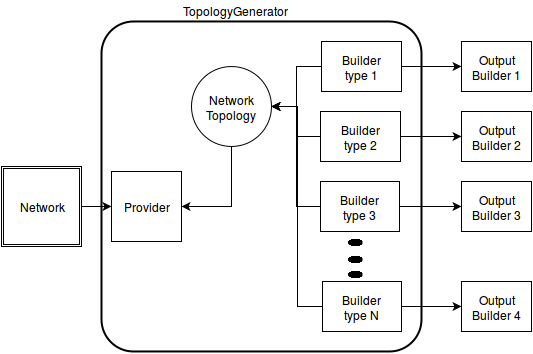
\includegraphics[width=\textwidth]{images/topologygenerator/topologygenerator_abstract_multiple.png}
\caption{Abstract interaction of elements with multiple outputs}
\end{figure}

In this image we can see how the elements explanied above interact. The provider will communicate with the real network, in the image above the real network is represented as the network which is outside the topology generator, to get all the information necessary in order to create the network topology representation. This comunication can either happen locally or remotely as we will see in one of the followings examples.\\
Once the representation is created, the builders are called to generate the output. In this example, we consider having N different types of elements in the network topology, which make us to have N different types of builders (1 per each type). Just to remark what was explained about the output, we are showing an example where we have one output per builder. This is not necessary the only case, as we can see in this other example: 

\begin{figure}[H]
\centering
\includegraphics[width=\textwidth]{images/topologygenerator/topologygenerator_abstract_single.png}
\caption{Abstract interaction of elements with single output}
\end{figure}

As we can see in this case, the logic of joining all the outputs from each of the builder's type is made by a new builder called TopologyBuilder, which is the one who finally generate's the desired output.\\

Now that we have a better understanding of the differents elements in the tool, we proceed to see some examples of use.

\subsection{Examples of use}

Let's consider now a concrete example where we want to obtain a network from either ONOS or OpenDayLight controller, and then create a DEVS's model for running simulations. We will assume that we are interested in hosts, devices and links of the network, meaning that we will consider only three types of elements. \\
In this example, we will need to have two providers, one per each controller, three builders, one per each type, and one more builder which will have the logic of joining all the output's provided to generate one common output, the topology.pdm, as show next:

\begin{figure}[H]
\centering
\includegraphics[width=\textwidth]{images/topologygenerator/controller_example.png}
\caption{Controller's example}
\end{figure}

Each of the providers in the image above, will have the knowledge to communicate with it's corresponding controller. In this example, the OnosProvider will encapsulate the logic to communicate with the Api Rest from the Onos controller, meanwhile the OpenDayLightProvider will do the same for the OpenDayLight controller.\\
The interaction with the controller can be either locally, for example this can happens if the controller is set up in the same machine where the topologygenerator is running, or remotely, for example if the controller is set up in a different machine and the comunication is made via http. How to implement both possibilities will be further explained in the next section.\\
The output generated is a pdm which can be interpretated by the DEVS simulator.\\

What happen if we do not have a real network?, What if we have a representation of a network in a programming language, for example Ruby, and we want to create from this network a simulation to test properties?. Then we can use the topologygenerator as follow in the next image:

\begin{figure}[H]
\centering
\includegraphics[width=\textwidth]{images/topologygenerator/ruby_provider.png}
\caption{Ruby as provider and DEVS as output}
\end{figure}
 
This image shows how it's just a question of creating a new provider, in this case the ruby provider, which will be in charge of having the knowledge of how to make the request to the script to obtain all the necessary information in order to create the network topology representation. Since we still want to create a simulation, the builders and the output is still the same. \\

In this previous example we show a powerful characteristic of the tool, which is that providers and builders are not related at all, meaning that changing a provider does not imply to change builders. This characteristic allow us then to create as much providers and builders as we want, and to connect them independently each other to generate as many desired output as we may want. \\

What would happend if we want to try out our custom topology written in Ruby, and test it in an Onos enviorment?, How could we manage to do this?.\\
In this example we would like to have our ruby provider, as in the previous case, and builders that generates request to the ONOS Api as show in the following image:

\begin{figure}[H]
\centering
\includegraphics[width=\textwidth]{images/topologygenerator/onos_builder.png}
\caption{Ruby as provider and ONOS as output}
\end{figure}

Each of the builder's in this case will generate requests to the ONOS Api that will create each of the elements in the SDN enviorment (this is a good example of the capability of SDN, since the enviorment allow us to create elements in the network). \\
In this example, it's important to notice how malleable and easy results to change ONOS, which was though as a provider in previous examples, to a desired output.\\

With the examples showed, we have a good understanding in the power of the tool and how it is supposed to be used. In the following section we will provide a tutorial for using the topologygenerator, and we will implement some of the examples showed before.

\section{Tutorial}

In this tutorial we will demonstrate how to install and use the topologygenerator tool. The tutorial was tested in a machine running Ubuntu 16.04, however should work in any machine which has a ruby version of 2.0 or major installed. \\

\subsection{Installation}

You will need to have Ruby installed in your machine. We recommend for this installing the ruby version manager (RVM), however any installation should be fine.\\

Once ruby is installed, you can proceed now to install the topologygenerator. For doing this, you will have two options: 
\begin{itemize}
\item Installing it as a gem \\
You should go for this option in case you are thinking in using the topologygenerator as a library of your Ruby project. 
\item Installing it as a binary \\
Select this option in case you are not interested in adding the topologygenerator as a library of any project. In this case, you will use the topologygenerator as a binary.
\end{itemize}

Per each option please refer to the corresponding subsection listed below.

\subsubsection{Installation as a gem}

Add this line to your application's Gemfile:

\begin{lstlisting}[language=Ruby,breaklines=true]
gem 'topologygenerator'
\end{lstlisting}

And then execute:

\begin{lstlisting}[language=bash,breaklines=true]
$ bundle
\end{lstlisting}

Or install it yourself as: 

\begin{lstlisting}[language=bash,breaklines=true]
$ gem install topologygenerator
\end{lstlisting}

\subsubsection{Installation as a binary}

\textbf{Pre-requisite}: Have installed and configured a git client. \\

Execute the followings lines (replace \textbf{TOPOLOGY\_DIRECTORY} with the corresponding path):

\begin{lstlisting}[language=bash,breaklines=true]
$ git clone git@github.com:andyLaurito92/topologygenerator.git
$ sudo ln -s "$TOPOLOGY_DIRECTORY/lib/createTopology.rb" /usr/bin/topologygenerator
\end{lstlisting}

\subsection{Using the tool}

How to use the topologygenerator will depend in which of the installation's guide you have done, however both ways are not so different and remember that you can always have the tool installed as a gem and a binary at the same time. In case you have installed the tool as a binary, we encourage you to first read the Use as a gem section, and then proceed to the Use as a binary section, since it still will be useful. \\
Both tutorials require you to have installed either Onos or OpenDayLight Controller and mininet. \\
First we will guide you in how to use the tool using the builders and providers implemented as examples, and then you will get hands on into the code and implement a provider and a builder. In both using examples, we will use the ONOS and OpenDayLight providers, and the PDM and Ruby builders. \\

NO ESTOY SEGURO SI SE PUEDEN USAR LOS BUILDERS Y PROVIDERS POR DEFECTO EN LA INSTALACIÓN DE LA GEMA, PORQUE NO SE SI RUBY TE DEJA ACCEDER A TODO EL PROYECTO DE LA GEMA, O SOLO AL BINARIO. TENGO QUE PROBAR ESTO, PERO EN CASO DE QUE NO SE PUEDA, ENTONCES EN LA INSTALACIÓN DE LA GEMA NO TENGO LOS BUILDERS Y PROVIDERS DE EJEMPLO, POR LO QUE TENGO QUE PENSAR EN COMO HACERLO ACCESIBLE PARA ESTOS MUCHACHOS.

\subsubsection{Use as a gem}

We will use the topologygenerator as a gem, meaning that will be part of your ruby code. \\
Using the tool is really straightforward, first we require the gem in the script as follows:

\begin{lstlisting}[language=Ruby,breaklines=true]
require 'topologygenerator'
\end{lstlisting}

And now we can create a new topologygenerator instance as follows:

\begin{lstlisting}[language=Ruby,breaklines=true]
my_topology_generator = TopologyGenerator.new({
        "source" => "ONOS", #Actually ONOS, OPENDAYLIGHT,  OBJECT and CUSTOM are the options supported
        "directory_concrete_builders" => "builders_examples/pdm_builders", #The directory where builders are located
        "output_directory" => "output_directory", #The directory where the output will be saved
        "uri_resource" => "http://127.0.0.1/onos/v1/" #Must be the rest api uri if either ONOS or OpenDayLight is choosed or the path of a file if CUSTOM is choosed. In case OBJECT is choosed, you will have to provide a valid instance of Topology.
    })
\end{lstlisting}

Let's go through the code in more detailed. What we are doing in this example is to tell the topologygenerator that we are going to use the ONOS provider, this is done just by passing as argument "ONOS" to the \textbf{source} key, and the DEVS builders, for doing this you just need to detailed the path where the builders are located to the \textbf{directory\_concrete\_builders} key. Since we have the topologygenerator gem installed, the enviorment has already loaded the path to the project, so there is no need to use the full path.\\
The next thing that you have to do is set the path where the output is going to be stored, for doing you just need to define the \textbf{output\_directory} key.\\
Finally since we are using the ONOS provider, we need to provide the uri from the ONOS's api. As you can see, this is done just by defining the \textbf{uri\_resource} key in the constructor. \\

After creating our topologygenerator instance, we can now proceed to generate the desired output by writing the following line in the code:

\begin{lstlisting}[language=Ruby,breaklines=true]
my_topology_generator.generate
\end{lstlisting}
 
The reader can have already noticed that what we are doing in this example, is implement the Controller's use case detailed in the previous section.\\

Before getting into the next example, let's go in more detailed in two of the four providers detailed above, the \textbf{CUSTOM} and \textbf{OBJECT} providers.\\
For using the \textbf{CUSTOM} provider, you will need to provide the path to the ruby network topology model file, which it would contain a valid model. Assuming that your model is in the following path: \textit{models/my\_network\_model/my\_network.rb}, this is how you have to create the topologygenerator's instance:

\begin{lstlisting}[language=Ruby,breaklines=true]
my_topology_generator = TopologyGenerator.new({
        "source" => "CUSTOM",
        "directory_concrete_builders" => "builders_examples/pdm_builders",
        "output_directory" => "output_directory",
        "uri_resource" => "models/my_network_model/my_network.rb"
    })
\end{lstlisting}

For further information of what is this model and how you can program one, please go ahead to the \textit{Network topology model} section.\\

For using the \textbf{OBJECT} provider, you will need to provide a valid instance of topology. Let's suppose that you have a variable called \textit{my\_topology} with a valid instance class, this is how you have to create your topologygenerator's instance:

\begin{lstlisting}[language=Ruby,breaklines=true]
my_topology_generator = TopologyGenerator.new({
        "source" => "OBJECT",
        "directory_concrete_builders" => "builders_examples/pdm_builders",
        "output_directory" => "output_directory",
        "uri_resource" => my_topology
    })
\end{lstlisting}

We encourage you to read more about the Topology class in the the topologygenerator API. In there you will be able to find examples in how to build a valid instance of this class.\\

Now that we have understood the providers, let's go trhough another example. Suppose that you want to use the tree topology network model located at \textit{network\_topologies\_examples}, for creating a simulation in PowerDevs. This is the way of doing this:

\begin{lstlisting}[language=Ruby,breaklines=true]
my_topology_generator = Topologygenerator.new({
        "source" => "CUSTOM",
        "directory_concrete_builders" => "builders_examples/pdm_builders",
        "output_directory" => "output",
        "uri_resource" => "network_topologies_examples/tree_topology.rb" 
    })
my_custom_topology = topology_generator.generate
\end{lstlisting}

What about if you want to use an OpenDayLight controller running in your local host, and from this network get a ruby representation model?. Then you will have to do as follow:

\begin{lstlisting}[language=Ruby,breaklines=true]
my_topology_generator = Topologygenerator.new({
        "source" => "OPENDAYLIGHT",
        "directory_concrete_builders" => "builders_examples/ruby_builders",
        "output_directory" => "output",
        "uri_resource" => "http://localhost:8080/restconf/operational/network-topology:network-topology/topology/flow:1/" 
    }) 
my_custom_topology = topology_generator.generate
\end{lstlisting}

As you may have already noticed, using the topologygenerator tool is really straightforward and flexible. We encourage you to keep on trying the tool with another builders and providers!. When you think that you are ready, you can jump on to code your first provider in the \textbf{Implementing your provider} section!.

\subsubsection{Use as a binary}

These are the commands that you need to know for using the topologygenerator as a binary:

\begin{itemize}
\item \textbf{-n (source name)} : The name of the provider. This can be matched with the source key in the topologygenerator's constructor in the previous section, but you have three providers instead of four (OBJECT is not supported in this way of use).
\item \textbf{-o (output directory)} : The path where the output will be stored. This can be matched with the output\_directory key in the topologygenerator's constructor in the previous section.
\item \textbf{-u (uri resource)} : A path to a ruby network model in case \textbf{CUSTOM} provider was selected, or an uri to an API if either \textbf{ONOS} or \textbf{OPENDAYLIGHT} were selected. This can be matched with the uri\_resource key in the topologygenerator's constructor in the previous section.
\item \textbf{-d (directory concrete builders)} : A path to a directory where the builders are located. This can be matched with the directory\_concrete\_builders in the topologygenerator's constructor in the previous section.
\end{itemize}

Remember that the path specified by argument can be relative, and in this case will be looked from the place where you are executing the command.\\

Suppose now that you want to use the topologygenerator for reading a network from ONOS, and build a simulation model. This is how you can do this:

\begin{lstlisting}[language=bash,breaklines=true]
$ topologygenerator source -n ONOS -o output_directory -u http://127.0.0.1/onos/v1/ -d builders_examples/pdm_builders
\end{lstlisting}

In case you want to try out the tree topology model for building a simulation, you can do it as follow:

\begin{lstlisting}[language=bash,breaklines=true]
$ topologygenerator source -n CUSTOM -o output_directory -u network_topologies_examples/tree_topology.rb -d builders_examples/pdm_builders
\end{lstlisting}

Or if you want to build a ruby model from an OpenDayLight network you can do the following:

\begin{lstlisting}[language=bash,breaklines=true]
$ topologygenerator source -n OPENDAYLIGHT -o output_directory -u http://localhost:8080/restconf/operational/network-topology:network-topology/topology/flow:1/ -d builders_examples/ruby_builders
\end{lstlisting}

Now that you know how to use the tool, let's proceed to get hands on and program your first provider!.

\subsection{Implementing your provider}

Provider's are one of the most important elements in the topologygenerator. Knowing how to implement a provider will give you the ability to extend the tool, and also to adapt the topologygenerator to your custom problem, are you ready to get started?. \\

In this tutorial we will show how to implement an OnosTopologyProvider, the only pre-requisite is to have ONOS installed either locally or remotely in order to test the implementation. \\

Every provider must inherit from a common interface called ITopologyProvider, this interface settles the methods that have to be implemented in the inherit classes. The methods mentioned are \textit{get\_topology} and \textit{get\_path\_between(source, destination)}


CAMBIAR LA IMPLEMENTACIÓN DEL PROVIDER PARA QUE SEA COMO LA DEL BUILDER!. SE PUEDE UTILIZAR LA YA CLASE IMPLEMENTADA CUSTOM Y CON ESTA HACER LO MISMO QUE HICIMOS CON EL ABSTRACT BUILDER.

\subsection{Implementing your builder}

As explained before, builders are the ones that will generate your desired output, but for doing this we first need to know what we we want as output!. In this example, we will implement the ruby builder which we have already been talking about (It's recommended that you have read \textbf{Network topology model} section before jumping into this tutorial). \\

We have already seen when we use the tool, that every time we called the topologygenerator, doesn't matter if it's as a binary or a gem, we have to specify a directory where the builders are located. In this directory, the topologygenerator will always try first to load a file called \textit{output\_concrete\_builder.rb}. This file has to contain a ruby module called \textbf{OtputConcreteBuilder}, with at least the following two methods: 
\begin{itemize}
\item \textit{initialize\_concrete\_builder}: This method will receive and instance of the topology provider being used in the ran, the path of the directory where the builders are (MAKE SENSES? WHY DID I DO THIS?) and the path of the output directory, that is where the desired output should be stored.
\item \textit{build\_output\_content}: This method will be called in the process of generation, and it's expected to generate the output in the specified folder.
\end{itemize}

So let's start then by creating a folder called \textit{ruby\_builders}, and creating in there our first file called \textit{output\_concrete\_builder.rb} . We already know some of the code that our file should have!, so let's start coding what we know up to know:

\begin{lstlisting}[language=Ruby,breaklines=true]
module OutputConcreteBuilder
	def initialize_concrete_builder(topology_provider, directory_concrete_builders, output_directory)
	end
    
    def build_output_content
    end
end
\end{lstlisting}

Great!, we have our base code. We know that our builder will generate a ruby model, and as how it was explained in the \textbf{Network topology model} section, this implies that we will be generating a module called \textit{NetworkTopology}, which will have to methods: \textit{get\_topology} and \textit{get\_path\_between(source,destination)}. This model that we are going to generate is going to be written in a file that we will call \textit{ruby\_network\_topology.rb}, and that we know that will be saved in the output directory. Using this knowledge let's start adding some generation code of what we know:

\begin{lstlisting}[language=Ruby,breaklines=true]
module OutputConcreteBuilder
	def initialize_concrete_builder(topology_provider, directory_concrete_builders, output_directory)
	end
    
    def build_output_content
    	ruby_network_topology = "module NetworkTopology \n"
    	ruby_network_topology += "    def get_topology \n "
    	ruby_network_topology += "    end \n "
    	ruby_network_topology += "    \n "
    	ruby_network_topology += "    def get_path_between(source,destination) \n "
    	ruby_network_topology += "    end \n "
    	ruby_network_topology += "end \n "
    end
end
\end{lstlisting}

We have just defined a variable called \textit{ruby\_network\_topology}, which will contain the content of our ruby model. Since know, we just defined the definition of the module, and the functions that we know that are going to be present. \\
An useful function for builders that the tool provides us is the \textit{write\_file} function. This function expect two arguments, first a string which would be the path where the file is going to be created in case it doesn't exist (it won't delete the file in case it already exsist), and second the content of the file to be created. In case the file already existed, the content will be overwritten.\\
Knowing that we can use this function, we can add the following lines to our \textit{output\_concrete\_builder.rb} file:

\begin{lstlisting}[language=Ruby,breaklines=true]
module OutputConcreteBuilder
	def initialize_concrete_builder(topology_provider, directory_concrete_builders, output_directory)
		@output_directory = output_directory
	end
    
    def build_output_content
    	ruby_network_topology = "module NetworkTopology \n"
    	ruby_network_topology += "    def get_topology \n "
    	ruby_network_topology += "    end \n "
    	ruby_network_topology += "    \n "
    	ruby_network_topology += "    def get_path_between(source,destination) \n "
    	ruby_network_topology += "    end \n "
    	ruby_network_topology += "end \n "
    	
    	write_file "#{@output_directory}/#{OUTPUT_RUBY_FILE_NAME}",
                    ruby_network_topology
    end
end
\end{lstlisting}

Two things were modified in the previous code, first the \textit{write\_file} function was added at the \textit{build\_output\_content} method, and the definition of the instance variable \textit{@output\_directory} was done in the \textit{initialize\_concrete\_builder} method. This instance variable was defined since we need to use it in the \textit{build\_output\_content} function. \\

Right now we have a builder which generates as output an empty, but still valid, ruby model. We want basically to create from the provider, which was given to us in the \textit{initialize\_concrete\_builder}, a network topology model. For doing this, we will need to get the elements of the network that the providers know, elements such as Host, Devices, Links, etc., and define this elements in our \textit{NetworkTopology} model. Some things to consider before keep going are: 
\begin{itemize}
\item We will just take into account the Host, Link and Router type in the Network. (Having different types as the mentioned above is not possible right know, however is not hard to extend the topologygenerator tool to have them. Please refer to the \textbf{Limitiations} section in this chapter for a better explanaition).
\item 
\end{itemize}

Understanding our assumptions and considerations, let's keep going in defining an instance variable for the \textit{topology\_provider} instance that we have recieved in the initialize function:

\begin{lstlisting}[language=Ruby,breaklines=true]
module OutputConcreteBuilder
	def initialize_concrete_builder(topology_provider, directory_concrete_builders, output_directory)
		@topology_provider = topology_provider
		@output_directory = output_directory
	end
    
    def build_output_content
    	ruby_network_topology = "module NetworkTopology \n"
    	ruby_network_topology += "    def get_topology \n "
    	ruby_network_topology += "    end \n "
    	ruby_network_topology += "    \n "
    	ruby_network_topology += "    def get_path_between(source,destination) \n "
    	ruby_network_topology += "    end \n "
    	ruby_network_topology += "end \n "
    	
    	write_file "#{@output_directory}/#{OUTPUT_RUBY_FILE_NAME}",
                    ruby_network_topology
    end
end
\end{lstlisting}

Now we can access the network topology elements from the \textit{build\_output\_content} function using the \textit{get\_topology} method from the \textit{topology\_provider} variable (as we have seen in the \textbf{Implementing your provider} section, all providers have defined this method). While doing this, we will get all the elements of type Host, Link and Router as mentioned above. 

\begin{lstlisting}[language=Ruby,breaklines=true]
module OutputConcreteBuilder
	def initialize_concrete_builder(topology_provider, directory_concrete_builders, output_directory)
		@topology_provider = topology_provider
		@output_directory = output_directory
	end
    
    def build_output_content
		network_elements = @topology_provider.get_topology
        
        network_elements = network_elements.select { |elem| [Host,Link,Router].include? elem.class }    
    
    	ruby_network_topology = "module NetworkTopology \n"
    	ruby_network_topology += "    def get_topology \n "
    	ruby_network_topology += "    end \n "
    	ruby_network_topology += "    \n "
    	ruby_network_topology += "    def get_path_between(source,destination) \n "
    	ruby_network_topology += "    end \n "
    	ruby_network_topology += "end \n "
    	
    	write_file "#{@output_directory}/#{OUTPUT_RUBY_FILE_NAME}",
                    ruby_network_topology
    end
end
\end{lstlisting}

The class Host, Link and Router are directly provided by the topologygenerator when the module is included. These classes have implemented a method called \textit{transform\_to\_output\_representation} which recieves as argument a path to a directory, and can be called to ask for an instance of this classes to be serialize. The calling of this method will triggered a loader which would try to load in the directories path provided as argument, a file name after it's class with "concrete\_builder.rb" appended at the end. For example, if we ask an instance of a host to be serialize (this means to call the method previous mentioned), the loader will try to load a file called \textit{Host\_concrete\_builder.rb} in the directory provide as argument. If the method is called by a Link's instance, the loader will try to load a file called \textit{Link\_concrete\_builder.rb}, and finally if the method is called by a Router's instance, the loader will try to load a file called \textit{Router\_concrete\_builder.rb}.\\
We show next what is the least expected content of these files:
\begin{lstlisting}[language=Ruby,breaklines=true,title=Router\_concrete\_builder.rb]
module RouterConcreteBuilder    
    def build_output_representation
    end      
end
\end{lstlisting}

\begin{lstlisting}[language=Ruby,breaklines=true,title=Host\_concrete\_builder.rb]
module HostConcreteBuilder    
    def build_output_representation
    end      
end
\end{lstlisting}

\begin{lstlisting}[language=Ruby,breaklines=true,title=Link\_concrete\_builder.rb]
module LinkConcreteBuilder    
    def build_output_representation
    end      
end
\end{lstlisting}

In each of the \textit{build\_output\_representation} functions is where you will have to program the code for serialize the instance. We will come back to this classes later. \\

Now that we have been provided of the network elements, it's time to define each of them as it is expected in the ruby model. Let's remember that in every ruby model we have the \textit{@topology} instance variable, which is the place in where we are supposed to add the network elements.\\
We first define three arrays, one per each type of element that we have in the topology. This arrays will be defined in the \textit{get\_topology} function of the ruby model as follow:

\begin{lstlisting}[language=Ruby,breaklines=true]
module OutputConcreteBuilder
	def initialize_concrete_builder(topology_provider, directory_concrete_builders, output_directory)
		@topology_provider = topology_provider
		@output_directory = output_directory
	end
    
    def build_output_content
		network_elements = @topology_provider.get_topology
        
        network_elements = network_elements.select { |elem| [Host,Link,Router].include? elem.class }    
    
    	ruby_network_topology = "module NetworkTopology \n"
    	ruby_network_topology += "    def get_topology \n "
    	ruby_network_topology += "       hosts = [] \n "
    	ruby_network_topology += "       routers = [] \n "
    	ruby_network_topology += "       links = [] \n "
    	ruby_network_topology += "    end \n "
    	ruby_network_topology += "    \n "
    	ruby_network_topology += "    def get_path_between(source,destination) \n "
    	ruby_network_topology += "    end \n "
    	ruby_network_topology += "end \n "
    	
    	write_file "#{@output_directory}/#{OUTPUT_RUBY_FILE_NAME}",
                    ruby_network_topology
    end
end
\end{lstlisting}

Now per each instance of elements that we are trying to add to the topology (let's remember that we have routers, hosts and links ), we will call the \textit{transform\_to\_output\_representation} method as follow:

\begin{lstlisting}[language=Ruby,breaklines=true]
module OutputConcreteBuilder
	def initialize_concrete_builder(topology_provider, directory_concrete_builders, output_directory)
		@topology_provider = topology_provider
		@output_directory = output_directory
		@directory_concrete_builders = directory_concrete_builders
	end
    
    def build_output_content
		network_elements = @topology_provider.get_topology
        
        network_elements = network_elements.select { |elem| [Host,Link,Router].include? elem.class }    
    
    	ruby_network_topology = "module NetworkTopology \n"
    	ruby_network_topology += "    def get_topology \n "
    	ruby_network_topology += "       hosts = [] \n "
    	ruby_network_topology += "       routers = [] \n "
	ruby_network_topology += "       links = [] \n "
	network_elements.each do |element|
		ruby_network_topology += "      #{element.transform_to_output_representation @directory_concrete_builders} \n"
        end
    	ruby_network_topology += "    end \n "
    	ruby_network_topology += "    \n "
    	ruby_network_topology += "    def get_path_between(source,destination) \n "
    	ruby_network_topology += "    end \n "
    	ruby_network_topology += "end \n "
    	
    	write_file "#{@output_directory}/#{OUTPUT_RUBY_FILE_NAME}",
                    ruby_network_topology
    end
end
\end{lstlisting}

As you can see, we have defined the new instance variable \textit{@directory\_concrete\_builders} for using it as argument to the \textit{transform\_to\_output\_representation} method. We now proceed to define each of the builder's class file per each type of element as it was explained above. We will explain in better detailed the \textit{Host\_concrete\_builder.rb} builder, and for the other's one we will give directly the code. 

\begin{lstlisting}[language=Ruby,breaklines=true,title=Host\_concrete\_builder.rb]
module HostConcreteBuilder    
    def build_output_representation
    	"hosts.push @topology.add_host \"#{id}\""
    end      
end
\end{lstlisting}

The code is straightforward, the function just add the host with it's corresponding id to the topology, and then pushes the result of this function to the hosts array previous defined. Notice that the function returns a string, since the idea is to serialize the host in the ruby model. \\
It's important to remark that the context in which this function is called, is the same as if it were a method defined in the Host class, meaning that we can access to every property and method defined in the Host class (in this case, we are accessing the id method). This behaviour is repeated in both \textit{Router\_concrete\_builder.rb} and \textit{Link\_concrete\_builder.rb}.\\

\begin{lstlisting}[language=Ruby,breaklines=true,title=Router\_concrete\_builder.rb]
module RouterConcreteBuilder    
    def build_output_representation
    	"routers.push @topology.add_router \"#{id}\", #{priority_weights}"
    end      
end
\end{lstlisting}

\begin{lstlisting}[language=Ruby,breaklines=true,title=Link\_concrete\_builder.rb]
module LinkConcreteBuilder    
    def build_output_representation
    	"links.push @topology.add_link \"#{id}\", #{src_element.id}, #{src_port}, #{dst_element.id}, #{dst_port}, #{bandwith}"
    end      
end
\end{lstlisting}

Remember that these files should be in the same folder as the \textit{output\_concrete\_builder.rb} file.\\

That's it!, you can now use your builder by specifying the path to the folder where the files are. You may have noticed that we didn't have implemented the \textit{get\_path\_between} method. This is something that we left you to do it with some helps:
\begin{itemize}
\item Is your topology static?, if it is, you may want just to hardcode the path between each of the hosts/routers in the network
\item Is your topology dynamic?, if it is you perhaps need to implement a search path algorithm like Dijkstra.
\end{itemize}

Hope you have understood everything and you are interested in making your own builders!. If that is the case, please don't hesitate to contact me to add them in the repository.

\subsection{Network Topology Model}

The Network Topology Model (NTM from now on), it's a way to model networks in the ruby language. It was invented to fulfill the need of describing all the elements in a network, meaning that we wanted to model not just the physical elements (as for example Hosts, Routers, Links, etc.), but also the abstract elements (flows and paths for example). The way of describing a network in this model is really straightforward, and is totally dependent on the topologygenerator tool (as we will see in the following section). \\
You should use this model everytime that you want to describe, test some properties (as you will find out in the following chapter), or just discover a network. \\
Now that you know what the NTM is and why it was program, go ahead to the implementing section and get your hands into the code!.

\subsubsection{Implementing your network topology model}

We will cover in this tutorial how we can manage to program our NTM for the following network 

\begin{figure}[H]
\centering
\includegraphics[width=300px]{images/topologygenerator/newtork_example.png}
\caption{Network to model}
\end{figure}

But first, let's understand the context in which we are going to use the model. \\

When you use the topologygenerator, between the provider's option there is one of the options that is \textit{CUSTOM}. This options is thought for recieving as uri's argument a path to a file where the NTM model will be program, meaning that the model which will be program in this tutorial will be used as resource of the topologygenerator. The NTM is a ruby module with \textit{NetworkTopology} as name, and two functions in it: \textit{get\_topology} and \textit{get\_path\_between(source, destination)}. The basic expected structure of this module is as follows:

\begin{lstlisting}[language=Ruby,breaklines=true]
module NetworkTopology
	def get_topology
	end
    
    def get_path_between(source, destination)
    end
end
\end{lstlisting}

Let's describe more into detailed both functions. The \textit{get\_topology} function will be the one, as it names remark, which will provide the network topology representation with all the elements described in the previous section (Host, Routers, Links, Paths, and Flows). This elements will have to be added to the instance variable \textit{@topology} which is already available in the module (to understand better why this happens, we encouraged the reader to study the \textit{CustomTopologyProvider} class from the \textbf{Appendix}).\\
The \textit{get\_path\_between(source,destination)} function will receive two instances from either Router or Host classes, and is expected to return an instance of Path with the corresponding path between both nodes (in case more than one exist, is the user responsability to select one). Since our network is harcoded, meaning that we already know the topological structure of it, this function will be trivial. \\

Let's describe then our desired topology. We have three hosts and one router, and every host will be connected to the router, and no host will be connected between each other. Let's first start by adding the routers and host to the topology.

\begin{lstlisting}[language=Ruby,breaklines=true]
module NetworkTopology
	def get_topology
		routers = []
        hosts = []

        router = @topology.add_router "MyRouter1"
        routers.push router

        for i in 0..2  
          host = @topology.add_host "Host#{i}"
          hosts.push host     
        end
	end
    
    def get_path_between(source, destination)
    end
end
\end{lstlisting}

Easy right?, we just need to add our elements with the desired properties to the topology and that's it!. We encouraged the reader to stop now this tutorial, and go and check the Topology api to see what properties can be set to each of the elements in the network. As you will se from the api, we are just setting the basics properties.\\
As you may have noticed, we have created two arrays, one per each element. This arrays will help us now in the creation of links, since we now have to create a link which has to receieve at least as argument it's source node, the port in which the link is connected in the source, it's destination node, and the port in which the link is connected in the destination node. By default adding a links is half duplex, meaning that if you want to have double communication you have either to add two links or use the \textit{add\_full\_duplex\_link} method from \textit{@topology}. In this example we will assume that we want the double connection, and we will use the first way of adding two links just to show how you should do this. The code will look as follow:

\begin{lstlisting}[language=Ruby,breaklines=true]
module NetworkTopology
	def get_topology
		routers = []
        hosts = []

        router = @topology.add_router "MyRouter1"
        routers.push router

        for i in 0..2  
          host = @topology.add_host "Host#{i}"
          hosts.push host     
        end
        
        #Links (starting from the flows that goes from top to bottom)    
        link1 = @topology.add_link "Link1", hosts[0], 0, routers[0], 0
        link2 = @topology.add_link "Link2", hosts[1], 0, routers[0], 1

        link3 = @topology.add_link "Link3", routers[0], 0, hosts[2], 0

        #Links (flows that goes from bottom to top)    
        link4 = @topology.add_link "Link4", hosts[2], 0, routers[0], 2

        link5 = @topology.add_link "Link5", routers[0], 1, hosts[0], 0
        link6 = @topology.add_link "Link6", routers[0], 2, hosts[1], 0
        
	end
    
    def get_path_between(source, destination)
    end
end
\end{lstlisting}

Here you can see how the host and router's arrays defined before take an important role for the link's definition. Looks a bit tricky at first, but if you stop a minute and see what we are doing here, is just to identify each host name per it's index, and then connect it to the router as we were supposed to by the model's image above. \\
This function must always return the elements of the topology, this is how you do it:

\begin{lstlisting}[language=Ruby,breaklines=true]
module NetworkTopology
	def get_topology
		routers = []
        hosts = []

        router = @topology.add_router "MyRouter1"
        routers.push router

        for i in 0..2  
          host = @topology.add_host "Host#{i}"
          hosts.push host     
        end
        
        #Links (starting from the flows that goes from top to bottom)    
        link1 = @topology.add_link "Link1", hosts[0], 0, routers[0], 0
        link2 = @topology.add_link "Link2", hosts[1], 0, routers[0], 1

        link3 = @topology.add_link "Link3", routers[0], 0, hosts[2], 0

        #Links (flows that goes from bottom to top)    
        link4 = @topology.add_link "Link4", hosts[2], 0, routers[0], 2

        link5 = @topology.add_link "Link5", routers[0], 1, hosts[0], 0
        link6 = @topology.add_link "Link6", routers[0], 2, hosts[1], 0
        
        @topology.topology_elements
	end
    
    def get_path_between(source, destination)
    end
end
\end{lstlisting}

And that's it for the \textit{get\_topology} function. We can now finish this tutorial by implementing our \textit{get\_path\_between(source, destination)} function. Like we said before, this would be really straightforward, since everyone is connected to everyone in either one or two steps!. This is an example of implementation of the get\_path function (and it's not the only possible!).

\begin{lstlisting}[language=Ruby,breaklines=true]
module NetworkTopology
	def get_topology
		routers = []
        hosts = []

        router = @topology.add_router "MyRouter1"
        routers.push router

        for i in 0..2  
          host = @topology.add_host "Host#{i}"
          hosts.push host     
        end
        
        #Links (starting from the flows that goes from top to bottom)    
        link1 = @topology.add_link "Link1", hosts[0], 0, routers[0], 0
        link2 = @topology.add_link "Link2", hosts[1], 0, routers[0], 1

        link3 = @topology.add_link "Link3", routers[0], 0, hosts[2], 0

        #Links (flows that goes from bottom to top)    
        link4 = @topology.add_link "Link4", hosts[2], 0, routers[0], 2

        link5 = @topology.add_link "Link5", routers[0], 1, hosts[0], 0
        link6 = @topology.add_link "Link6", routers[0], 2, hosts[1], 0
        
        @topology.topology_elements
	end
    
    def get_path_between(source, destination)
    	first_link = @topology.topology_elements.select { |elem| (elem.is_a? Link) && (elem.src_element == source) }.first
        second_link = @topology.topology_elements.select { |elem| (elem.is_a? Link) && (elem.dst_element == destination) }.first

        path = Path.new(source,destination)        
        path.add_link first_link
        path.add_link second_link unless first_link.dst_element == destination
        path
    end
end
\end{lstlisting}

In this implementation we are just looking for the links that match the source and destiny nodes, add the first link always, and check if the second link should be added (remember that we can be asked by a host and router's path, which in this case means that only one link should be added). \\

Congratulations!, you have implemented your first ruby NTM!, you can now go ahead and check it out, and start playing around with the example programed. In the next subsection we will cover how to add Paths with Flows in the network implemented.

\subsubsection{Adding Paths with Flows}

We will cover now how to add paths and flows in the following context: Suppose that we are thinking on setting up the enviorment previous model, this means buying all the equipment for the hosts, thinking in which would be the best links for the network, which type of router should we buy?. \\
This type of questions are usually made in the setting up of any network enviorment, and are usually answered with statistics of the network traffic, assumptions of traffic generation from each of the elements in the network, etc. This network trafic assumptions, or even the network traffic statistics most of the times can be aproximated by mathematical's distribution, and uniting this knowldge with DEVS, we can easily simulate a NTM by just describing it's characteristics in this model, and then generating the DEVS's model for running a simulation. Using then the previous model, and the assumption that each of the hosts will generate traffic following an exponential distribution, and the size of the packets will follow a constant distribution, we can add three flows per host as follows:

\begin{lstlisting}[language=Ruby,breaklines=true]
module NetworkTopology
	def get_topology
		routers = []
        hosts = []

        router = @topology.add_router "MyRouter1"
        routers.push router

        for i in 0..2  
          host = @topology.add_host "Host#{i}"
          hosts.push host     
        end
        
        #Links (starting from the flows that goes from top to bottom)    
        link1 = @topology.add_link "Link1", hosts[0], 0, routers[0], 0
        link2 = @topology.add_link "Link2", hosts[1], 0, routers[0], 1

        link3 = @topology.add_link "Link3", routers[0], 0, hosts[2], 0

        #Links (flows that goes from bottom to top)    
        link4 = @topology.add_link "Link4", hosts[2], 0, routers[0], 2

        link5 = @topology.add_link "Link5", routers[0], 1, hosts[0], 0
        link6 = @topology.add_link "Link6", routers[0], 2, hosts[1], 0
        
		flow_1_path = Path.new hosts[0], hosts[2]
        flow_1_path.add_link link1
        flow_1_path.add_link link3
        @topology.add_flow "Flow1", 
                            10, 
                            [flow_1_path], 
                            (ExponentialDistribution.new 1.0/6875), 
                            (ConstantDistribution.new 1000*8)

        flow_2_path = Path.new hosts[1], hosts[2]
        flow_2_path.add_link link2
        flow_2_path.add_link link3
        @topology.add_flow "Flow2", 
                            15, 
                            [flow_2_path], 
                            (ExponentialDistribution.new 1.0/6875), 
                            (ConstantDistribution.new 1000*8)

        flow_3_path = Path.new hosts[2], hosts[1]
        flow_3_path.add_link link4
        flow_3_path.add_link link5
        @topology.add_flow "Flow3", 
                            20, 
                            [flow_3_path], 
                            (ExponentialDistribution.new 1.0/6875), 
                            (ConstantDistribution.new 1000*8)         
        
        @topology.topology_elements
	end
    
    def get_path_between(source, destination)
    	first_link = @topology.topology_elements.select { |elem| (elem.is_a? Link) && (elem.src_element == source) }.first
        second_link = @topology.topology_elements.select { |elem| (elem.is_a? Link) && (elem.dst_element == destination) }.first

        path = Path.new(source,destination)        
        path.add_link first_link
        path.add_link second_link unless first_link.dst_element == destination
        path
    end
end
\end{lstlisting}

Let's explain in more detailed what we are doing in the \textit{Flow1} definition (this explanaition will cover all the three flow's definitions).\\
What we first do is define a path between two hosts in this line: 

\begin{lstlisting}[language=Ruby,breaklines=true]
flow_1_path = Path.new hosts[0], hosts[2] 
\end{lstlisting}

The first one correspond to the flow's source, and the next one corresponds to the flow's destination. We then add a valid path between both nodes, and we finally use the \textit{add\_flow} method from the Topology class to define a new flow between these nodes. If you want a better explanaition of each of the arguments received by the function, we encouraged you to read the \textbf{Topology} API.

\section{Limitations}

\section{Future work}

There are a lot of things that still need to be done in this tool:

\begin{itemize}
\item Extend the SDN Controllers provider's for retrieving more information\\
The information fetched now in the tool is enough, but we are not taking advantage of all the information that we had!. Could we define flows using the entities flow that exist in each of the controllers?, Do they represent the same concept?, Could we define the flow distribution's just by using controller's statistics?
\item Adapt the providers to have the same behaivour as builders\\
Providers and builders are very similar in code as you have already seen. Both should be implemented in the same way, and having the builder's implementation for providers will allow a better extensibility of the tool, since now we are limited to the providers that exist, and adding or modifying a provider implies changing the tool code. 
\item Add more providers and builders \\
The number of providers and builders that are now implemented is really small. Providers that would be interest to have would be: a provider for the \textit{Topology Zoo} topologies \cite{topologyzoo}, another for InfiniBand \cite{infiniband}, Can this last provider be done?, What changes would it imply?. In the other hand, it would be interest to have builders for the controller's, for OMNeT++ \cite{omnet} in order to extend the reacheability of the tool
\item Allow the posibility to extend network entities\\
If we can manage to allow the user to extend the network entities, or even use different entities, we would make the tool much more abstract and powerful. What would be needed for doing this?, Can we do something similar as we did with the builders?
\item Add more abstract entities\\
\item Extend the Network Topology Model 
\end{itemize}

\chapter{Haikunet}
\section{Conceptual Idea}

Haikunet is a SDN programming langauge which was created with the main objective of fulfilling the need of debugging the network, and creating an intent's oriented programming language agnostic to the controller. This last property means that Haikunet will not be coupled to a particular controller at all. Right now OpenDayLight and ONOS are the Controller's supported, but as you will see in following sections, enlarge this number is not hard at all, and you will have the chance to do this by following the tutorial.\\
Writing programs in Haikunet is really easy and straightforward, and this language will give you the advantage of having just one intent written in a common way for several controllers, something that up to now you weren't able to do as far as the writers of this thesis know.\\
The language is interpretated, written in Ruby and can be ran in any machine with a Ruby major or equal version of 2.0.0. This is how a program written in Haikunet looks like:

\begin{lstlisting}[language=Ruby,breaklines=true]
one_host := Host(mac="9A:4A:43:D4:36:45", vlan="-1", ipAddresses=["10.0.0.1"], elementId="of:0000000000000002", port="4")

second_host := Host(mac="72:D2:0D:24:C5:36", vlan="-1", ipAddresses=["10.0.0.4"], elementId="of:0000000000000003", port="4")

my_flow := Flow (src=one_host, dst=second_host, priority="55")

Intent firstExample
	Select my_flow
\end{lstlisting}

This program describes an intent for creating a flow between two host. We will come back to explain in more detailed this program and all the elements involve in the \textbf{Learning Haikunet} section.\\

The main ideas that you have to understand before writing a program in this language are the followings:

\begin{itemize}
\item Initial Topology\\
Which would be the initial topology?, think of this as the network in which you want to apply the intent. It's called initial because it can be seen as the initial point from where we start, and after the intent is applied to the newtork, we will obtain the desired network, which can be called the last one. In the \textbf{Formal Definition} section this is better explained.
\item What is what you want from the newtork?\\
Try to understand well what are you going to ask to the network, if it's possible to do it, which components are going to be involved in, etc. From this though, you will write your program.
\item Which is going to be the destiny?\\
Has the destiny the ability to do what you are expecting from the network?. Remember that you can always debug first what you are doing, and then proceed to apply it to the real network!.
\end{itemize}

After this, as every programming language, you will need to practice in order to write good programs. Let's take a look at the architectural components of the language, and how they relate one with each other.

\begin{figure}[H]
\centering
\includegraphics[width=\textwidth]{images/haikunet/arquitectura_haikunet.png}
\caption{Haikunet architectural view}
\end{figure}

The components in the left are the arguments the interpreter expect (except the topologygenerator tool which is a gem used by the language). We will come back in more detailed to these arguments in the \textbf{Learning Haikunet} section.\\
Inside the black box are the components which make up the interpreter, these will be explained in more detailed at the \textbf{Implementation} section, and finally at the right are the possible outputs that the language can provide (ONOS and OpenDayLight component's represent a generation of a bunch of request to one of these controllers, DEVS is the generation of the .pdm file, and finally ERROR represents that something went wrong while interpretating the program). These will also be seen in the \textbf{Learning Haikunet} section.\\

As it can be apreciated in the image, Haikunet uses the topologygenerator tool which was explained in the previous chapter. The topologygenerator gives an important characteristic to the language, which is that it allows us to create a NTM model and use it as our intial network, meaning that it's not mandatory to have a real network for using Haikunet. Another important thing is one of the destinies which Haikunet support's, DEVS. Supporting this destiny gives the language an important characteristic, which is permiting to simulate from either a real network or a NTM model how would an intent react in the initial newtork.\\

Haikunet flow's work as follow: We first run the interpreter giving as argument a progam and an output destiny, this output destiny specifies to which controller the program is being interpretated. The interpreter lexer's then receive the program, which will be in charge of tokenize it and give it to the parser, which will detect if the tokens are gramatically well written. After this, the semantic checker will detect either statical or dynamical errors in the program (we will explain in more detailed this erros definition's in the \textbf{Formal Definition} section), using the underlaying network which was given by the topologygenerator tool. After this two things can happen: either the program had no errors, meaning that the code generator will execute the bunch of request that have to be done to the API of the controllers specified in the input of the interpreter, or it had, this will cause an error raise exception with a message which will explain the problem. \\

This short paragraph resumes the working flow of a program being interprated by Haikunet. In the \textbf{Language Implementation} section we will cover in detailed what happens in each of the components previously mentioned.\\

Now that we have a better idea of what Haikunet is, let's proceed to give some formal definition's before getting into the tutorial, but before this let us explain you something.

\section{Why Haikunet?}

The name Haikunet comes from the join of Haiku and Network. A Haiku is a Japanese poem with a lot of themes, but in most of the cases a Haiku describes the nature from the view of an observer. This is exactly what you are going to do with Haikunet, write short programs which will describe the desired nature of a network, and this description will be done from the point of view of an observer of the network, meaning a person which does not necessarily knows how to interact at a system level with it, and in most of the cases, doesn't know how to. This is the intent's programmer point of view of the network. 

\section{Formal Definition}

In this section we will establish key concepts and main ideas that will be use in this chapter. The section will be divided in one definition after another, and after all definitions are made, we will continue with the Haikunet tutorial.\\

\subsection{Debugging}

Debugging will be the process of finding either static or dynamic errors before the intent is applied to the network. The definition of these type of erros can be found ahead in the section.\\
In this work, we are not going to explore techniques which involves stopping an intent execution's in a controller. 

\subsection{Error}

An error will be a request made by a program written in Haikunet, which has not semantically sense in the context of the current network. Since this definition involves a huge amount of errors for a thesis work, we will focus in a limited scope which will be introduced next. We will show some scenarios, their respectively errors in them, and the error output that the interpreter will show:

\subsubsection{Flow property definition error}

\textbf{Description:} This error happens when you use a host property in a flow definition, and this property cannot be neither found or inferred from the initial network topology. \\

\textbf{Example:} Let's suppose that we have the following initial network:

\begin{figure}[H]
\centering
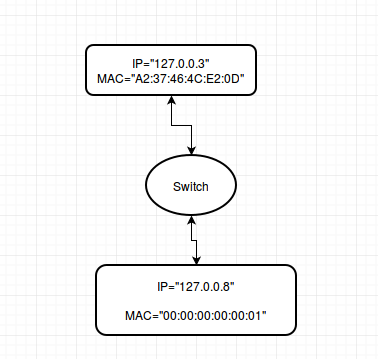
\includegraphics[width=\textwidth]{images/haikunet/error_scenario_1.png}
\caption{Initial network context in flow property definition error}
\end{figure}

and we execute the following program:

\begin{lstlisting}[language=Ruby,breaklines=true]
source_host := Host(mac="A2:37:46:4C:E2:0D")

my_flow := Flow (src=source_host, dst="127.0.0.10", priority="55")

Intent firstExample
    Select my_flow
\end{lstlisting}

In this example, we have the problem that the property \textit{dst = "127.0.0.1"} is not a valid ip in the current network. \\

An important observation here is that this is an error, because the mistake is made in the flow definition line. If we would have a mispelled property in the Host definition as we show in this example (let's assume that I wanted to create a flow between \textit{127.0.0.3} and \textit{127.0.0.8}):

\begin{lstlisting}[language=Ruby,breaklines=true]
source_host := Host(ip="127.0.0.2")

my_flow := Flow (src=source_host, dst="127.0.0.8", priority="55")

Intent firstExample
    Select my_flow
\end{lstlisting}

This would not be considered as an error, since the semantic of this program in the initial network context given before, would mean first to create a host with \textit{127.0.0.2} as IP, and then create a flow between this new host and the one which has \textit{127.0.0.8} as IP.

\subsubsection{No path error}

\textbf{Description:} This error is thrown when you are trying to create a flow between two host which have no path between them.

Let's suppose that we have the following initial network:

\begin{figure}[H]
\centering
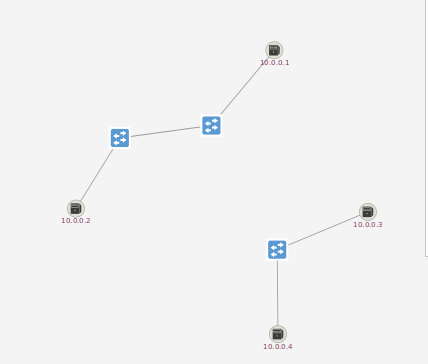
\includegraphics[width=\textwidth]{images/haikunet/error_scenario_2.png}
\caption{Initial network context in no path error}
\end{figure}

and we execute the following program:

\begin{lstlisting}[language=Ruby,breaklines=true]
source_host := Host(ip="10.0.0.2")

    destiny_host := Host(ip="10.0.0.4")

my_flow := Flow (src=source_host, dst=destiny_host, priority="55")

Intent firstExample
    Select my_flow
\end{lstlisting}

It can be seen in the image above that the error is thrown because there is no path between hosts \textit{10.0.0.2} and \textit{10.0.0.4}. 

\subsubsection{Inconsistent host definition error}

\textbf{Description:} This error is thrown when you are trying to either create or refer to a Host which already exist with different properties from the real ones. 

Let's suppose that we have the following initial network:

\begin{figure}[H]
\centering
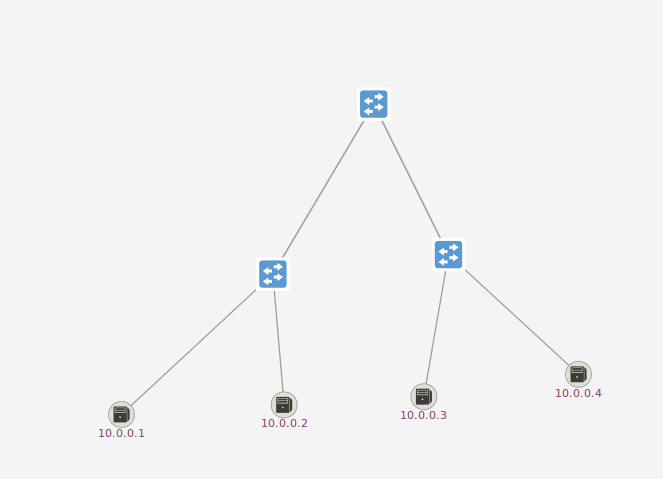
\includegraphics[width=\textwidth]{images/haikunet/error_scenario_3.png}
\caption{Initial network context in inconsistent host definition error}
\end{figure}

and we execute the following program:

\begin{lstlisting}[language=Ruby,breaklines=true]
one_host := Host(mac="9A:4A:43:D4:36:45", vlan="-1", ipAddresses=["10.0.0.1"], elementId="of:0000000000000002", port="1")

second_host := Host(mac="72:D2:0D:24:C5:36", vlan="-1", ipAddresses=["10.0.0.4"], elementId="of:0000000000000003", port="2")

my_flow := Flow (src=one_host, dst=second_host, priority="55")

Intent firstExample
    Select my_flow
\end{lstlisting}

The problem here is that we are trying to define the same host with different mac addresses. CORRECT THE IMAGE SO WE CAN SEE THE HOST WITH ITS CURRENT MAC.

\subsubsection{Percentage in loss packets error}

STILL HAS TO BE IMPLEMENTED.

\subsection{Static and Dynamic errors}

When debugging definition was made, static and dynamic errors were mentioned. We now proceed to define each type of error, and we will categorize the erros showed before in order to understand better these definitions.

\begin{itemize}

\item Static error\\
A static error can be defined as an error which can be pointed out as one, without the need of letting time pass into the underlying network. Examples of these types of erros showed before are the \textit{Flow property definition error}, \textit{No path error} and \textit{Inconsistent host definition error}
\item Dynamic error\\
A dynamic error can be defined as an erorr which needs time to be elpased in the underlying network, in order to identify it as one. An example of this kind of error is the \textit{Percentage in loss packets error}. 
\end{itemize} 

As it can be seen on the definition above, time is a variable needed for defining both kind of errors. This variable is introduced because the network is a model which is always changing, and not necesarilly just because a program changes it (for example we can always have either infraestracture or software issues, making links and host not reacheable, causing a change in the underlying network topology).\\
From the definition of both types of erros, we studied the best way to detect each of them.\\
From the first type of errors, an interpreter using a network model plus a definition of a semantic checker were implemented in order to detect them.\\ Since for detecting the second type of errors we need time to be elapsed in the underlying network, and the time needed varies depending on each error, a connection with DEVS was implemented. The key idea in this is having a representational model of the network, which can be ran as a simulation in DEVS, modelling hours of time elapsed in the network. The simulation will then replied with results, and from this results we will be able to detect if there are dynamic errors present in the program. 


\subsection{Initial Network}

The concept of initial network comes from the following view: When you apply an intent to a network, you can see the network as a mutable element which is being transformed by the application of an intent. This abstraction allow us to identify different network states that can be pointed out in the intents process: The first one, the initial one, is the network in which the user wants to apply the intent. Then there is a last one, which is the one in which the intent has already been applied, in case it was possible to do so, and is the newtork result of applying the intent. Since the intent can transform several times the network (for example first adding a host, then adding a link, etc.), we can identify all the intermediate states in which the network has to be in order to reach the last state. \\
From the given approach, in the \textbf{Future work} section we will introduce several ideas that we have related to this important concept.

\section{Language Implementation}

This section is focused to describe how each of the components detailed in the Haikunet architectural view is implemented, we will follow the processing flow as it was explained in the \textbf{Conceptual Idea} section, and start explaining how is both the lexer and parser implemented.

\subsection{Lexer/Parser}

For a better understanding of these two components, we need first to introduce the grammar of the language. 

\subsubsection{Haikunet Grammar}

The grammar of the language is as follows:

\begin{lstlisting}[breaklines=true]
Start ->	New_Network_Definition | New_Intent

New_Network_Definition ->	Identifier := Network_Elem_Def

Identifier ->	[.:A-Za-z0-9_-]+

Sring ->	[.:A-Za-z0-9_-]+

Network_Elem_Def ->	Abstract_Elem_Def | Concrete_Elem_Def

Abstract_Elem_Def ->	Action_Def | Flow_Def | Condition_Def

Concrete_Elem_Def ->	Host_Def | Link_Def | Device_Def 

Host_Def ->	Host( Params )

Link_Def ->	Link( Params )

Device_Def ->	Device( Params )

Action_Def ->	Action( Params )

Flow_Def ->	Flow( Params )

Condition_Def ->	Condition( Params )

Params -> 	Identifier = Identifier, Params | 
			Identifier = Identifier |
			Identifier = "String", Params |
			Identifier = "String" |
			Identifier = Array_Identifiers, Params |
			Identifier = Array_Identifiers 

Array_Identifiers ->	[ Elems_Of_Array ] 

Elems_Of_Array ->	Identifier  | Identifier, Elems_Of_Array

New_Intent ->				Intent Identifier
			Select Identifier	
			|    
			Intent Identifier
				Select Identifier            	
				Action Identifier                    
			| 
			Intent identifier
				Select Identifier
				Action Identifier
				Condition Identifier
\end{lstlisting}

It can be seen here that Haikunet is though for either defining the elements of the network, or defining the intent. The elements that can be defined are either concrete elements, where concrete stands up for defining elements which have a phisical representation in the network, as for example a Host, a Link and a Device, or abstract elements, where abstract represent elements as the flow, an action and a Condition. \\
For defining whatever type of element in the language, we just need to create an identifier, which will represent our element in the entire execution of the program, and define the element name in camelcase follow by the parameters needed for the creation. The nonterminal Parameters is describing to us that there is not an only way of defining an element in the language, so a question comes up which is, how should we define an element?. The answer to this question relies on the destiny of the program, and will be treated in the \textbf{Code Generation} section. \textbf{PODRÍAMOS PENSAR EN UNA FORMA DE DEFINIR CHEQUEOS SEMANTICOS DEPENDIENDO DEL DESTINY, PUES LA DEFINICIÓN DE PARAMETROS ESTA TOTALMENTE SUBEDITADA A ESTO.}

Actions and conditions are elements which are intended to be as parameters of the intent definition, and are think to work as follows:
\begin{itemize}
\item Action PENSAR MEJOR\\
An action represents a change to be done in every element that matches the identifier provided. For example, if we have the following intent definition:
\begin{lstlisting}[language=Ruby,breaklines=true]
one_host := Host(mac="9A:4A:43:D4:36:45", vlan="-1", ipAddresses=["10.0.0.1"], elementId="of:0000000000000002", port="1")

drop_packets := Action(from="9A:4A:43:D4:36:45", realize="DROP")

Intent firstExample
    Select one_host
    Action drop_packets
\end{lstlisting}

We are saying that every packet that is sent from \textit{one\_host} should be dropped. The possible actions allowed are: CUALES SON? PENSAR QUE ES LO QUE QUIERO MODELAR
\item Condition PENSAR MEJOR\\
A condition represents the act of monitoring a property in the network, and measure it in the scale detailed in the condition definition. It is always used with an action, and when the condition is satisfied, the action is performed. This is an example of use of a condition:
\begin{lstlisting}[language=Ruby,breaklines=true]
one_host := Host(mac="9A:4A:43:D4:36:45", vlan="-1", ipAddresses=["10.0.0.1"], elementId="of:0000000000000002", port="1")

one_device := Device(mac="9C:B1:C2:D4:36:12")

drop_packets := Action(from="9A:4A:43:D4:36:45", realize="DROP")

measure_of_loss_packets := Condition(one_device.packets_loss > 0.5)

Intent firstExample
    Select one_host
    Action drop_packets
    Condition measure_of_loss_packets
\end{lstlisting}
What we are doing in this case is to set an intent which describes what to do when a device starts to lose more than the 50\% of traffic. In this case, when the condition is satisfied, we start dropping packets of the host with IP \textit{10.0.0.1}.
\end{itemize}

Now that we have a better understanding of the grammar of the language, we can come back to explain in more detailed how the lexer was implemented.

\subsubsection{Lexer}

The lexer is in charge of recieving the program, and tokenize it's content. The tokens that we have identified from the grammatic presented above are the following ones: 
\begin{itemize}
\item \textbf{END\_OF\_LINE}\\
As it names points out, this token will be replaced every time the string \textit{\\n} is found
\item \textbf{EQUAL\_PARAMETERS}\\
This tokens represents the equal which is put in the paramateres definition, between parenthesis.
\item \textbf{LEFT\_PARENTHESIS}\\
This token represents the character \textit{(}
\item \textbf{RIGH\_PARENTHESIS}\\
This token represents the character \textit{)}
\item \textbf{DOUBLE\_QUOTE}\\
This token represents the character \textit{"}
\item \textbf{LFET\_BRACE}\\
This token represents the character \textit{[}
\item \textbf{RIGHT\_BRACE}\\
This token represents the character \textit{]}
\item \textbf{COMMA}\\
This token represents the character \textit{,}
\item \textbf{ASSIGN}\\
This token represents the characters \textit{:=}
\item \textbf{HOST}\\
This token represents the definition of a \textit{Host} element. The language does not take into account if the name was written in either upper case or lower case or a cambination of these.
\item \textbf{LINK}\\
This token represents the definition of a \textit{Link} element. The language does not take into account if the name was written in either upper case or lower case or a cambination of these.
\item \textbf{DEVICE}\\
This token represents the definition of a \textit{Device} element. The language does not take into account if the name was written in either upper case or lower case or a cambination of these.
\item \textbf{FLOW}\\
This token represents the definition of a \textit{Flow} element. The language does not take into account if the name was written in either upper case or lower case or a cambination of these.
\item \textbf{INTENT}\\
This token represents the definition of a \textit{Intent} element. The language does not take into account if the name was written in either upper case or lower case or a cambination of these.
\item \textbf{SELECT}\\
This token represents the definition of a \textit{Select} element. The language does not take into account if the name was written in either upper case or lower case or a cambination of these.
\item \textbf{ACTION}\\
This token represents the definition of a \textit{Action} element. The language does not take into account if the name was written in either upper case or lower case or a cambination of these.
\item \textbf{CONDITION}\\
This token represents the definition of a \textit{Condition} element. The language does not take into account if the name was written in either upper case or lower case or a cambination of these.
\end{itemize}

This lexer was implemented with the lookahead character thecnique, and can be seen as the following state machine:

\begin{figure}[H]
\centering
\includegraphics[width=\textwidth]{images/haikunet/lexer_state_diagram.png}
\caption{Lexer as a state machine}
\end{figure}

Once the lexeme is tokenize, the parser component will be in charge of detect if the program is well written. Let's see how this component was implemented.

\subsubsection{Parser}

The parser implemented for the grammatic previously described is an LL(1). Since the grammar showed before is not LL(1) friendly (since the nonterminals \textit{Params}, \textit{Elems\_of\_array} and the \textit{Initial\_simbol} make the parsing with one look ahead impossible in this context), we had to rewrite it as follows:

\begin{lstlisting}[breaklines=true]
Start -> Identifier := Network_Elem_Def     | Intent Identifier Select Identifier Intent_Prod_With_Action

Intent_Prod_With_Action ->	Action Identifier Intent_Prod_With_Condition | Lambda

Intent_Prod_With_Condition ->	Condition Identifier | Lambda

Identifier	->	[.:A-Za-z0-9_-]+

Sring	->	[.:A-Za-z0-9_-]+

Network_Elem_Def	->	Host(Params)| Link(Params)| Device(Params) | Action(Params) | Flow(Params) | Condition(Params)

Params	->	Identifier= Second_part_Equal | Lambda

Second_part_Equal	->	"String" Add_more_parameters | Identifier Add_more_parameters |  [ Elems_Of_Array ]  Add_more_parameters 

Add_more_parameters	->	,Params | Lambda

Elems_Of_Array	->	Identifier Add_more_elems_to_array | "String" Add_more_elems_to_array 

Add_more_elems_to_array	->	, Elems_Of_Array | Lambda

\end{lstlisting}

It can be easily checked that this grammar generates the same language that the one detailed before. The only new element which is present in this grammar is the \textit{Lambda} nonterminal, which represents the empty string.\\
Besides detecting programs which are not well formed, in the parser we implement the logic of constructing the abstract syntax tree, which will be used for the code generator for creating the desired output. For doing this, we extended the previous grammar to a sytax-directed translated grammar as show next:

\begin{lstlisting}[breaklines=true]
Start	->	Identifier := Network_Elem_Def  
	{
		identifiers.push(Identifier.new Identifier)
		identifiers[Identifier].val = Network_Elem_Def
	}  
|
Intent Identifier1 Select Identifier2 Intent_Prod_With_Action 
	{     
		action_and_condition = Intent_Prod_With_Action
		intents.push (Intent.new identifier1);
		intents[identifier1].select = identifier2
		intents[identifier1].action = action_and_condition['action']
		intents[identifier1].condition = action_and_condition['condition']
	}
	
Intent_Prod_With_Action	->	Action Identifier Intent_Prod_With_Condition 
		{ 
			identifier_condition = Intent_Prod_With_Condition
			return {'action':Identifier, 'condition':identifier_condition}
		}
| 
     Lambda
        {
            identifier_condition = Intent_Prod_With_Condition
            return {'action':NONE, 'condition':identifier_condition}
		}

Intent_Prod_With_Condition	->	Condition Identifier 
    {
        return Identifier
	}
| 
Lambda
    {
        return NONE
	}

Identifier	->	[.:A-Za-z0-9_-]+

Sring	->	[.:A-Za-z0-9_-]+

Network_Elem_Def	->	Host(Params)
    {
		actual_params = [ ] 
		return Host.new Params 
	}
| 
Link(Params)
    { 
    	actual_params = [ ] 
		return Link.new Params 
	}
| 
Device(Params) 
	{ 
		actual_params = [ ] 
		return Device.new Params 
	}
| 
Action(Params) 
    { 
    	actual_params = [ ] 
		return Action.new Params 
	}
|
Flow(Params)
    { 
	    actual_params = [ ] 
		return Flow.new Params 
	}
| 
Condition(Params)
    { 
	    actual_params = [ ] 
		return Condition.new Params 
	}

Params	->	Identifier= Second_part_Equal 
    { 
		actual_identifier = Identifier.new Identifier
		Second_part_Equal
	}
| 
Lambda
    {
        return actual_params
    }

Second_part_Equal	->	"String" Add_more_parameters 
    { 
        actual_identifier.val = "String"
		actual_params.push actual_identifier
		Add_more_parameters
	}
| 
Identifier Add_more_parameters 
    {
        actual_identifier.val = Identifier
		actual_params.push identifiers[actual_identifier]
		Add_more_parameters
	}
|  
[ Elems_Of_Array ]  Add_more_parameters 
{
    elems_of_array = []
    actual_identifier.val = Elems_Of_Array
	actual_params.push identifiers[actual_identifier]
	Add_more_parameters
}

Add_more_parameters	->	,Params 
    {
        Params
	}
| 
Lambda
    {
        
    }

Elems_Of_Array	->	Identifier Add_more_elems_to_array 
    { 
		elems_of_array.push identifiers[Identifier]
		Add_more_elems_to_array
 }
| 
"String" Add_more_elems_to_array 
    {
        elems_of_array.push Identifier
		Add_more_elems_to_array
    }

Add_more_elems_to_array	->	, Elems_Of_Array 
    {
        Elems_Of_Array.
	}
| 
Lambda
    {
        return elems_of_array
    }
\end{lstlisting}

Ruby is the code showed above in the extended grammar.\\
After having our program parsed, the next step is to check if the program is semantically correct. For doing this, we have implemented a semantic checker which will be explained next. 

\subsection{Semantic Checker}

\subsection{Code Generation}

\section{Tutorial}

\subsubsection{Installation}

\textbf{Pre-requisite:} You need to have a git client installed, a machine running a Linux distribution (it was tested in an Ubuntus machine, but should work in any Linux distribution machine), and already installed a ruby version equal or major to 2.0.0.

For installing Haikunet, just run the following commands:

\begin{lstlisting}[language=bash,breaklines=true]
$ git clone git@github.com:andyLaurito92/haikunet.git
$ cd haikunet
$ sudo ./install_haikunet.sh 
\end{lstlisting}

And that's it!, you have already installed the interpreter. Let's understand a bit more about the language before jumping into the code.

\subsubsection{Using the interpreter}

\textbf{Pre-requisite:} Have running locally the ONOS controller, and have already download the language repository.

For running the Haikunet interpreter, you will need: 
\begin{itemize}
\item The path to the file where the haikunet program is (remember that only files with the ".hk" extension are allowed).
\item Specify one of the destinations supported (the current supported are \textit{ONOS}, \textit{OPENDAYLIGHT} and \textit{DEBUG}).
\item An URI from where to obtain the initial topology.
\end{itemize}

Let's get into more detailed in the last two arguments.\\
The destination argument is an option which will tell the interpreter to which destiny has to generate the code of the input program, the options current supported are \textit{ONOS}, \textit{OPENDAYLIGHT} and \textit{DEBUG}. The first two are controllers, and selecting one of them will generate a bunch of request to the corresponding API REST. The DEBUG option will generate a simulation in DEVS, taking as initial topology the one specified by argument, and will show you simulations result's once the run is complete. The idea is that with this results, you will be able to identify if the network behaviour is the one you expected. We will get into more detailed on this in the \textbf{Implementing your first program} subsection.\\
The other argument is the URI from the Initial Network, which was already explained in the \textbf{Formal Definition} section. As the name remarks, will be either a URI of an API REST of a controller, or a path to a file which will contain a ruby NTM (this was explained in the previous chapter, in the \textbf{Network Topology Model} section).\\

Let's now suppose that:
\begin{itemize}
\item We want to execute the \textit{host\_to\_host.hk} program (you can find it in \textit{\$HAIKUNET\_DIRECTORY/examples/programs}), which creates two host if they don't exist in the underlying network, and creates a flow between them. 
\item We are using ONOS as destiny output.
\item We will use as initial topology the one that we have at ONOS. 
\end{itemize} 

This is how you use the interpreter for doing that (we will assume that you will execute the haikunet interpreter from the \textit{\$HAIKUNET\_DIRECTORY}, and the ONOS local version that you are running can be located at http://127.0.0.1:8181 address):

\begin{lstlisting}[language=bash,breaklines=true]
$ haikunet program -n examples/programs/host_to_host.hk -d ONOS -u http://127.0.0.1:8181/onos/v1/
\end{lstlisting}

In the previous command:
\begin{itemize}
\item \textbf{-n} is the option to provide the path to the interpreter.
\item \textbf{-d} is the destiny name.
\item \textbf{-u} is the path to the uri initial topology.
\end{itemize}

If you want to debug the same program using the same initial topology, just run the following command:

\begin{lstlisting}[language=bash,breaklines=true]
$ haikunet program -n examples/programs/host_to_host.hk -d DEBUG -u http://127.0.0.1:8181/onos/v1/
\end{lstlisting}

You may also want to try to use as initial topology the one provided in \textit{examples/initial\_topologies} to debug it. The command to run in this case is:

\begin{lstlisting}[language=bash,breaklines=true]
$ haikunet program -n examples/programs/host_to_host.hk -d DEBUG -u examples/initial_topologies/example_topology.rb
\end{lstlisting}

In case your default controller is OpenDayLight, you just have to use the OPENDAYLIGHT destiny, and specify the uri \textit{http://OPEN\_DAY\_LIGHT\_IP:8080/restconf/operational/network-topology:network-topology/topology/flow:1/}, where \textit{OPEN\_DAY\_LIGHT\_IP} stands for the corresponding IP address of the controller. 

You can find these and more examples in the interpreter help's by running the following command:

\begin{lstlisting}[language=bash,breaklines=true]
$ haikunet program --help
\end{lstlisting}

Now that we know how to use the interpreter, let's write our first program!.

\subsubsection{Implementing your first program}

\subsection{Implementing your CodeGenerator}

\section{Future work}

\chapter{Conclusions and Future Work}
\input{conclusions.tex}

%%%% BIBLIOGRAFIA
\backmatter
\bibliography{tesis}
\begin{thebibliography}{9}
\bibitem{topologyzoo} 
http://www.topology-zoo.org, \textit{The Internet Topology Zoo}, University of ADELAIDE 

\bibitem{topologyzoo} 
https://omnetpp.org/, \textit{OMNeT++}

\bibitem{infiniband} 
http://www.mellanox.com/pdf/whitepapers/IB\_Intro\_WP\_190.pdf, \textit{Introduction to InfiniBand}, Mellanox Technologies, White Paper


\end{thebibliography}

\end{document}
